%Write MapGenerator explanation

In this simulator, the world consists of a map with two main types of cells; movable and immovable cells. Movable cells are the objects that an agent can move in or through and consist of pathways, doors, targets, sentry towers, and shade areas, where the immovable cells only involve inner and outer walls. It is assumed that agents can walk underneath sentry towers. The following section explains the methods used to generate the maps that were used in the experiments.
Every method starts by placing the outer walls; walls that surround the whole map and that do not hold doors nor windows. Next they generate all the other walls and the doors and windows on these walls. Consequently, the movable objects are placed on the map at the desired places.

\subsubsection{SplitRoom}
The $SplitRoom$ algorithm takes the full map and splits it in two at an arbitrary point, so two separate rooms are created. It takes the created rooms and splits them as well. It continues splitting the small rooms until either the maximum amount of splits is reached. Accordingly, it takes all the rooms and places two doors on each wall, hence, the agents will always find ways to leave and enter every room in multiple ways.
The $SplitRoom$ algorithm is created in two different versions, the original $SplitRoom$ and the $RandomSplitRoom$ algorithm. The original $SplitRoom$, splits alternating horizontally and vertically. The $RandomSplitRoom$ algorithm splits the rooms with a random orientation.
\begin{figure}[H]
\centering
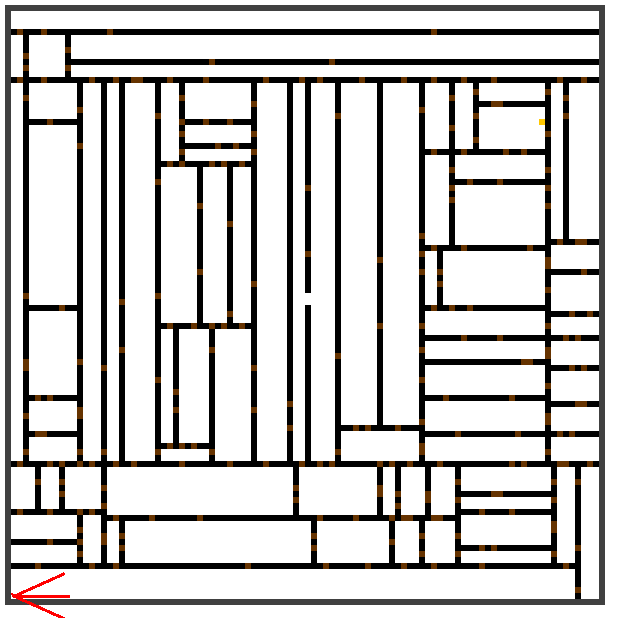
\includegraphics[width=\columnwidth]{images/randomRoom.png}
\caption{Example of map generated by $RandomSplitRoom$.}
\label{fig:maze05}
\end{figure}

\subsubsection{URoom}
The $URoom$ algorithm places U-shaped walls on random locations and with random rotations on the map, until the set amount of U-shaped walls is reached.
The $StaticURoom$ algorithm divides the whole map into subsections and places U-shaped walls of the same sizes but different rotations in these subsections.
As the implementation of these algorithms does not allow closed rooms, the placement of doors is not implemented in this method.
\begin{figure}
\centering
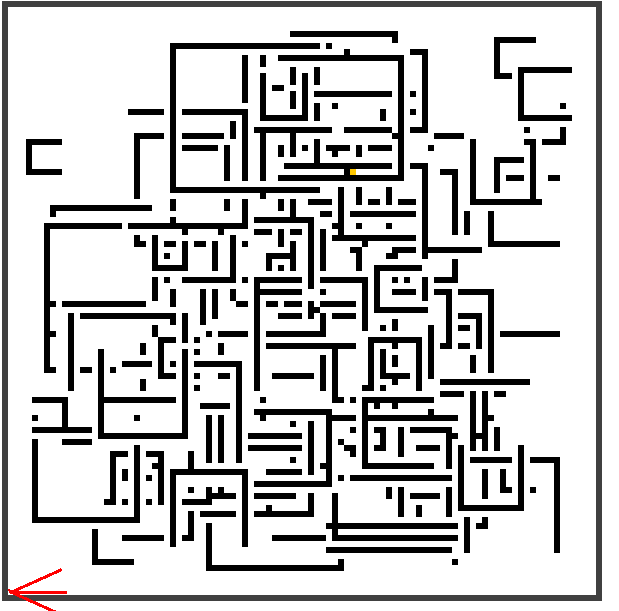
\includegraphics[width=\columnwidth]{images/uroom.png}
\caption{Example of map generated by $URoomGenerator$}
\label{fig:uroom}
\end{figure}

\subsubsection{Maze}
The maze-type map is generated by starting with a map that is completely filled with walls. Then a spanning tree of open tiles is generated starting from a random tile using Prim's algorithm \cite{graham1985history}. This will ensure that there is only one possible path from any open tile to any other open tile. To generate maps of varying complexity walls are removed randomly to create more possible paths to the goal. At complexity $1$, no additional walls are removed, and at complexity $0$ all walls are removed. The complexity is thus the proportion of walls removed after a spanning tree has been created.
\begin{figure}[H]
\centering
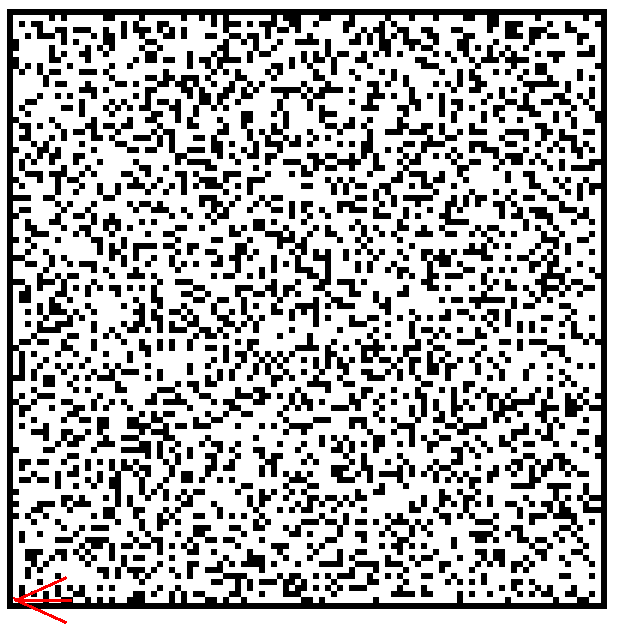
\includegraphics[width=\columnwidth]{images/maze05.png}
\caption{Example of map generated by $MazeGenerator$ with complexity 0.5.}
\label{fig:maze05}
\end{figure}

\begin{figure}[H]
\centering
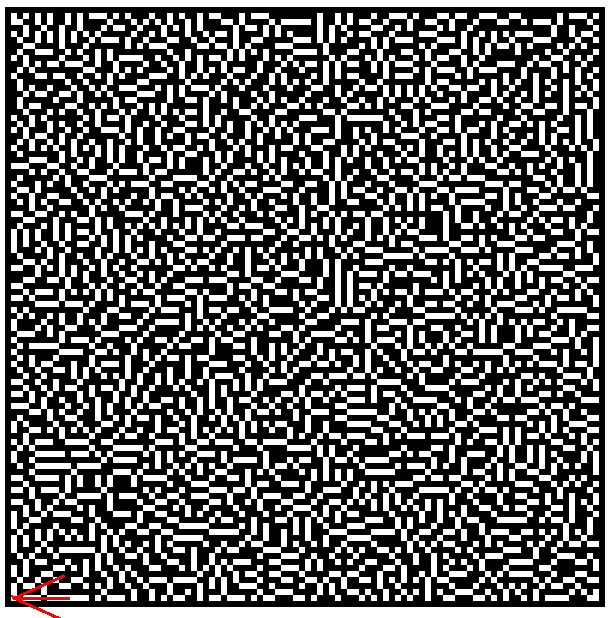
\includegraphics[width=\columnwidth]{images/maze1.png}
\caption{Example of map generated by $MazeGenerator$ with complexity 1.0.}
\label{fig:maze1}
\end{figure}
